\section{Architecture}\label{sec:architecture}

The architecture of LAOS is discussed in detail in
Section \ref{sec:arch-highlevel}, after an initial
discussion of a key separation pattern of asset ownership 
and asset attributes used all across LAOS in Section \ref{sec:separation}.
Section \ref{sec:architecture-future}
concludes with the vision beyond the initial implementation.


\subsection{The Ownership-Attributes Split}\label{sec:separation}

At the core of the technology is a hard separation
between asset ownership and asset attributes, brought to the extreme
whereby both sets of data can live and be managed by different blockchains,
but carefully designed to be properly linked, 
and allow for on-chain traceability and certification.

Unlike traditional NFTs, where both sets are either stored on-chain
in the same blockchain's contract, or where the attributes are stored
in external, static, content-addressed systems (pattern \bref{eq:tokenURIIPFS})
or in external, privately-owned servers (pattern \bref{eq:tokenURICentral}),
LAOS separation allows both sets of data to live in different decentralized {\it 
consensus systems}.

\begin{Figure}
    \medskip
    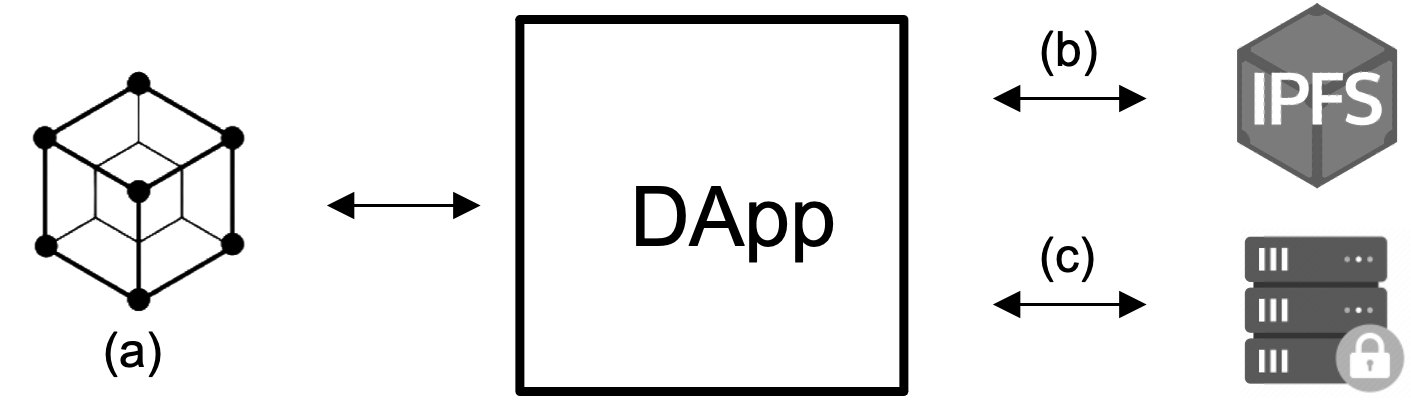
\includegraphics[width=1\textwidth]{patterns.png}
    \captionof{figure}{
        Typical structure of nodes/services required to run a DApp, such as a marketplace:
        (a) a consensus node, e.g., an Ethereum node; (b)
        an IPFS node, for NFTs implementing pattern \bref{eq:tokenURIIPFS}; (c)
        access to privately-owned internet servers, for NFTs implementing pattern \bref{eq:tokenURICentral}.
    }
    \medskip
    \label{fig:patterns}
\end{Figure}

Figure \ref{fig:patterns} illustrates the traditional NFT node structure to which
DApps normally connect. While DApp developers
have the choice to operate their own consensus nodes,
particularly for fully permissionless blockchains,
it is commonplace to rely on third-party node providers that
ensure consistent uptime and handle maintenance \cite{stogerdemystifying}.
Likewise, developers often opt to use third-party IPFS providers to guarantee 
that content is pinned with high data availability.

\begin{Figure}
    \medskip
    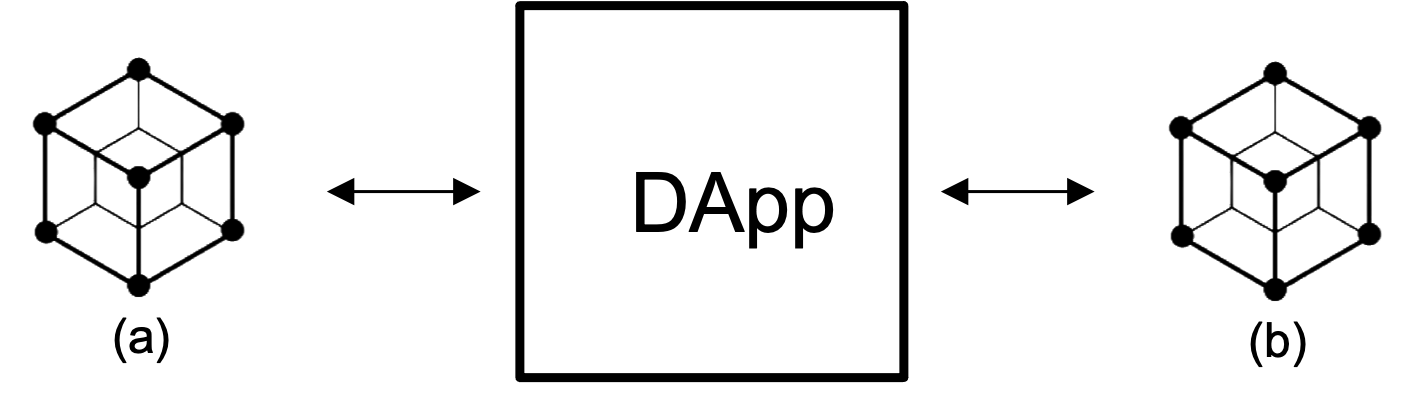
\includegraphics[width=1\textwidth]{patterns_2nodes.png}
    \captionof{figure}{
        Structure of nodes when implementing the ownership-attributes split,
        with a DApp using two different consensus nodes, one for ownership (a)
        and one for attributes (b).
    }
    \medskip
    \label{fig:patterns2nodes}
\end{Figure}

Figure \ref{fig:patterns2nodes} shows the structure for patterns
based on LAOS' ownership-attributes split, whereby only consensus nodes are
required. Figure \ref{fig:patterns2nodesAs1} shows a convenient architecture
where the DApp only interacts with one single node, which can be built permissionlessly:
the node maintains a state that internally syncs with the two consensus system,
and exposes a single API that abstracts all complexity, and mimics a single ERC721/1155
compliant system. 

\begin{Figure}
    \medskip
    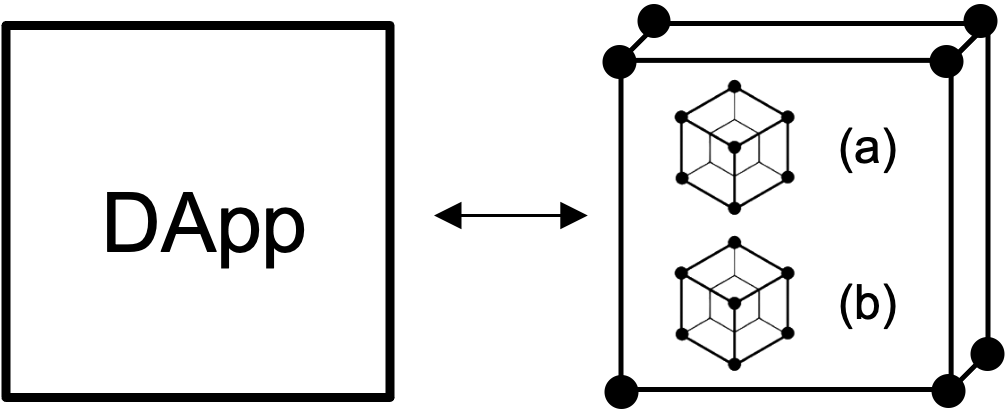
\includegraphics[width=1\textwidth]{patterns_2nodesAs1.png}
        \captionof{figure}{
            A convenient way to structure nodes in ownership-attributes split patterns,
            where a DApp interacts via the ERC721/1155 standard interface 
            with one single node that abstracts all complexity.
        }
    \medskip
    \label{fig:patterns2nodesAs1}
\end{Figure}

The link between both consensus systems can be achieved by using recently developed standards
like the {\it Universal Location} pattern, introduced as part of XCMv3 by
Polkadot, and described in more detailed in section \ref{sec:universal-location}.
From the point of view of the patterns described in section \ref{tokenURI},
this standard enables the DApps to reference assets that live in different
consensus systems:
\bea
\label{eq:tokenURIConsensus}
\mbox{tokenURI:} \mbox{ tokenId} &\rightarrow & \mbox{Consensus Address} 
\eea 

This fundamental aspect, as well as the design to link both systems,
is reflected the LAOS architecture detailed in the next
sections, and sits at the core of the bridgeless minting \& evolution feature
discussed in Section \ref{sec:bridgeless-tech}.

\subsection{High-level architecture}\label{sec:arch-highlevel}


\subsubsection{Leveraging Polkadot's ecosystem and features}

LAOS is architected as a specialized Parachain in Polkadot\cite{polkadot}, \cite{polkadotExplained},
fully devoted to providing the ideal platform to fulfill the aforementioned Living Assets requirements and vision.
The architectural design choices exploit several benefits that are unique to Polkadot, among others:
\begin{itemize}
    \item as a Parachain, it will automatically inherit the full security guarantees 
    provided by Polkadot's Relay Chain from day 1;
    \item by internally being built on Substrate and using the GRANDPA\footnote{GRANDPA stands for GHOST-based Recursive Ancestor Deriving Prefix Agreement, a finality gadget for consensus systems originally presented in\cite{grandpa}.}
    consensus algorithm, it will also share top features such as non-probabilistic
    fast block finality, and forkless upgrades of its protocol;
    \item it will make use of Polkadot's recently introduced Universal Location pattern, as part of XCMv3;
    \item it will heavily leverage other Parachains in the ecosystem, making it easy to interact
    with EVM-compatible smart contracts, guarantee long-term data availability, access to DeFi, and
    benefitting from a combined maximum transactions per second (TPS) estimated between 100K and 1M;
    \item it will allow its internal design to leverage Polkadot's developed Relay Chain 
    and trustless bridges technology to achieve, mid-term, a scalability comparable to second order relay chains.   
\end{itemize}

As side benefits, Polkadot's available rich set of tools and open code bases will
allow LAOS to avoid reinventing the wheel, use battle-tested software,
and progressively adopt upgrades developed by other teams, while contributing to the ecosystem.

\subsubsection{Components}

LAOS will by built around the architecture depicted in \fig{fig:architecture}.
We hereby detail its main system components.

\vspace{\baselineskip}

{\bf (a) Relay Chain.}
At the root of the LAOS consensus protocol is Polkadot's Relay Chain, with the set 
of Polkadot validators that provide security to the Parachain, ensuring that
every transaction processed by a Parachain is valid. The Relay Chain
also help Parachains transfer assets and connect functionalities in a fully
trustless way via native Cross-Consensus Messaging (XCM), and efficiently 
linking the light clients that Parachains have from other Parachains.

\vspace{\baselineskip}

{\bf (b) LAOS Ownership Parachain.}
The LAOS Ownership Parachain will be a specialized chain, based on the 
Polkadot standard NPoS protocol, with the following functionalities:
\begin{itemize}
    \item host and manage the LAOS native utility token;
    \item manage the ownership of all LA created directly in LAOS, with 
    transactions implemented at the protocol level,
    and fees paid in the native tokens;
    \item manage runtime upgrades of all Evolution Chains (Evochains);
    \item store state roots of the Evochains, exposing asset attributes
    certification methods,
    and reward Evochains validators upon reception of new correct roots;
    \item manage all trustless transfers of Living Assets and LAOS tokens
    between LAOS and the rest of Parachains via XCM;
    \item implement and coordinate governance and staking.
\end{itemize}

\begin{Figure}
    \medskip
    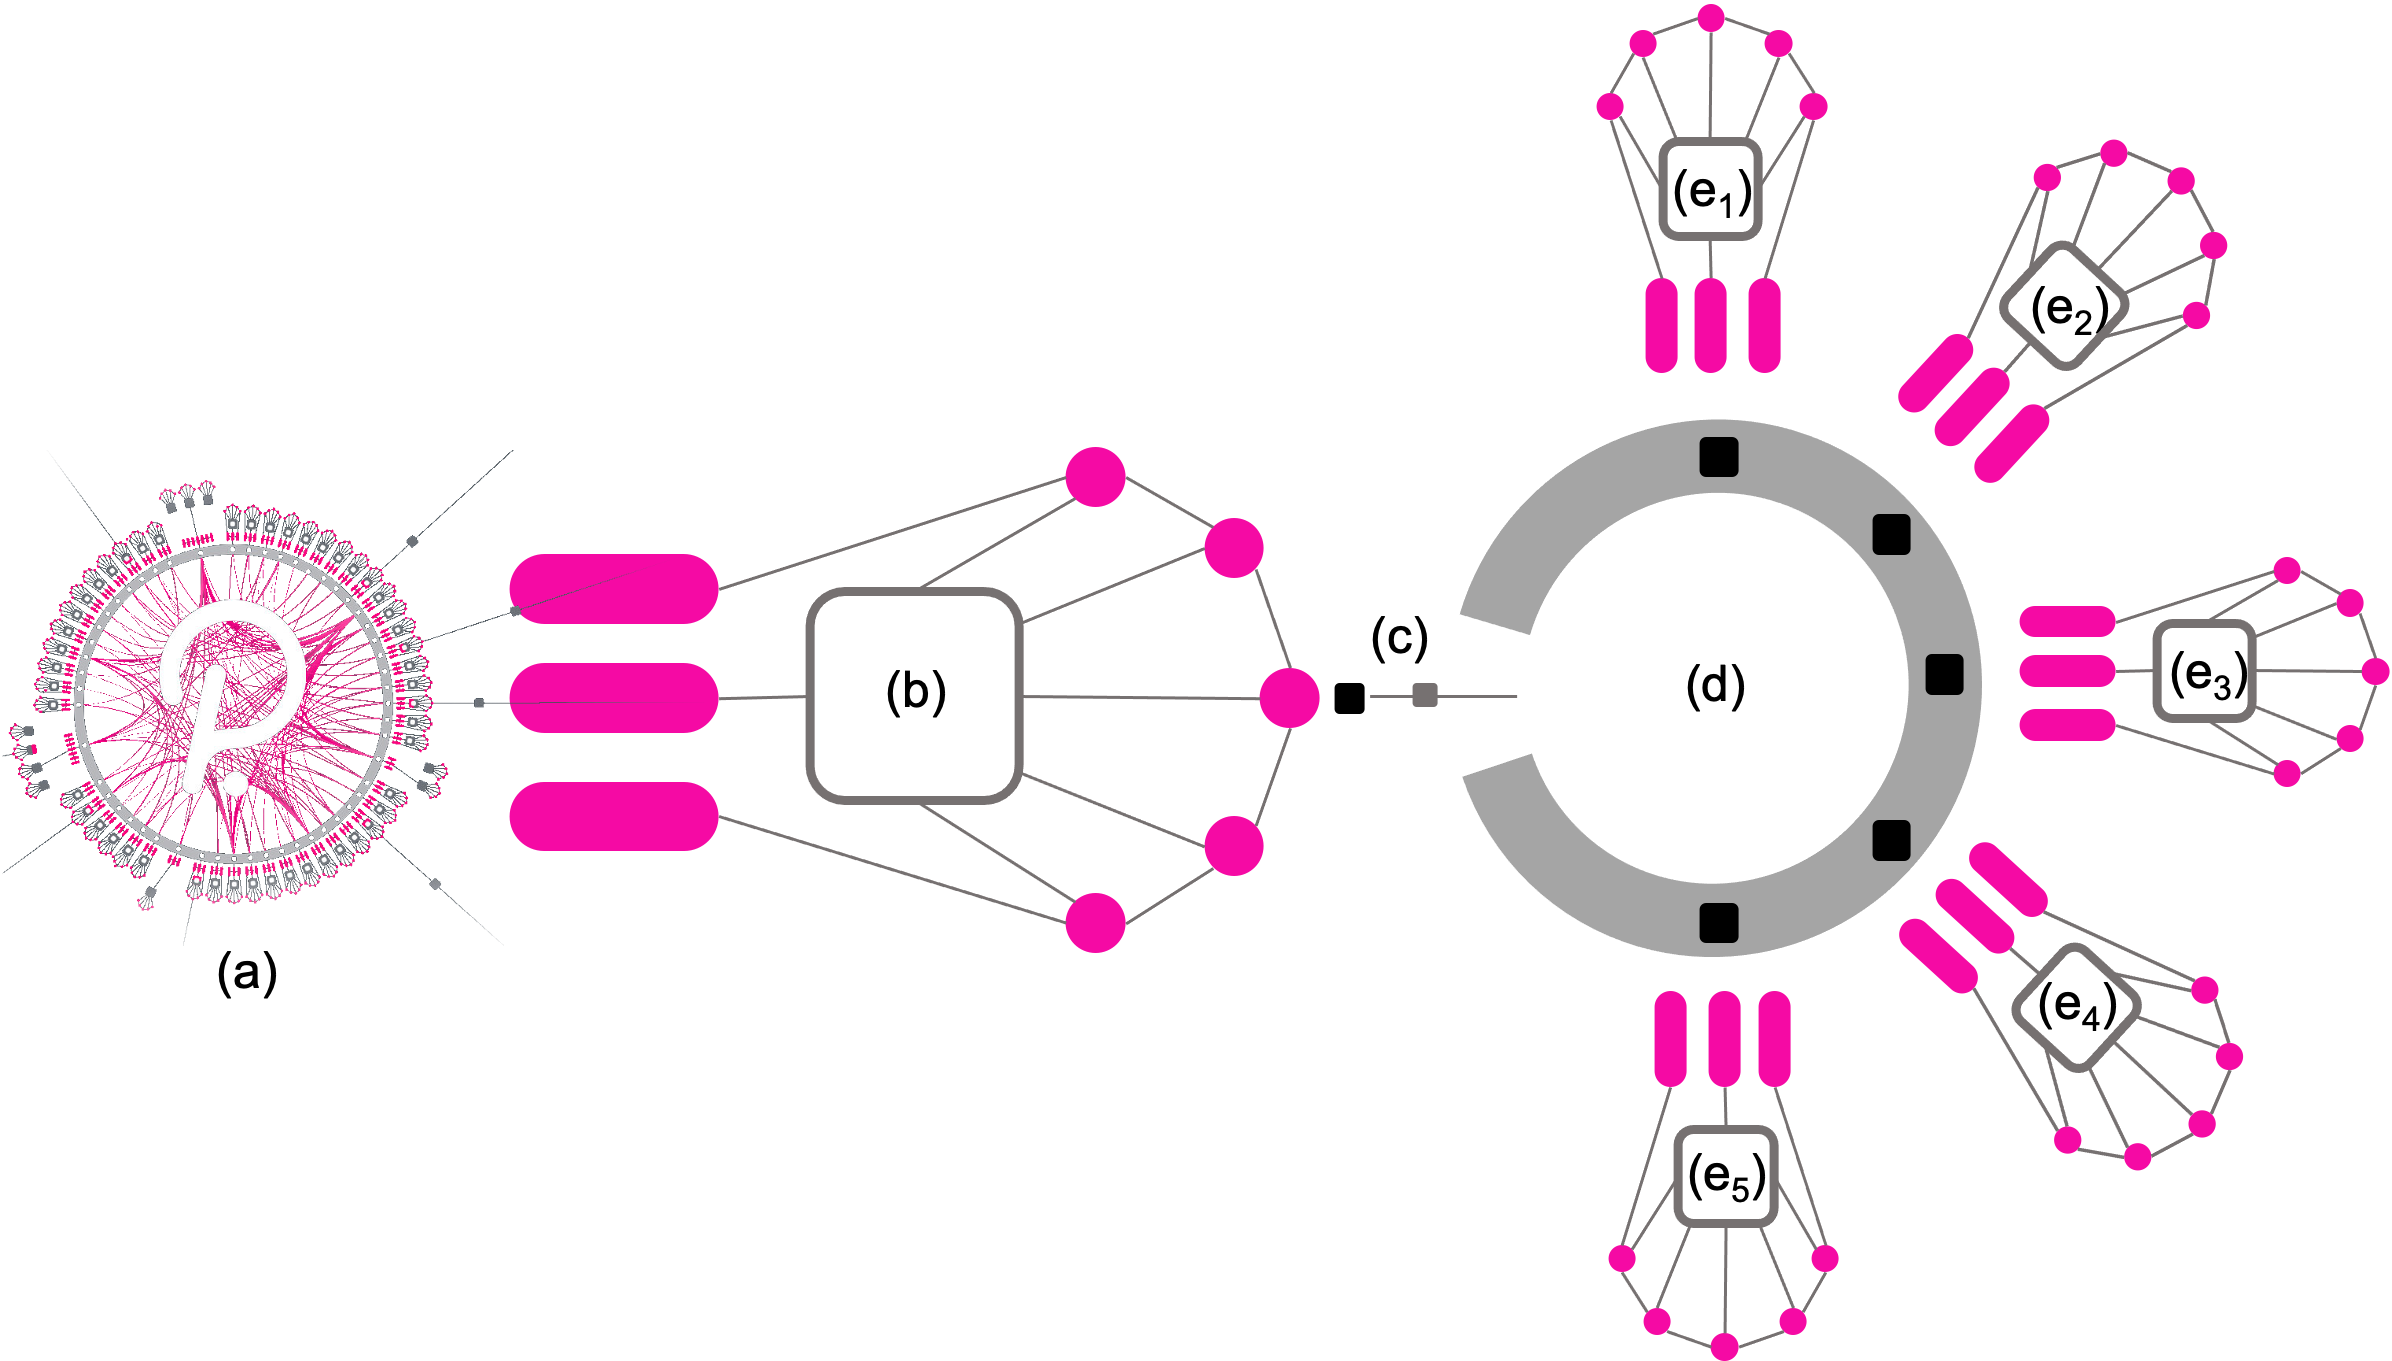
\includegraphics[width=1\textwidth]{laos-architecture.png}
    \captionof{figure}{High-level architecture of LAOS, containing: (a) Polkadot's relay
    chain, (b) the LAOS ownership Parachain, (c$_i$) the LAOS Evochains, 
    (d$_i$) the trustless bridges connecting Evochains to the ownership Parachain }
    \medskip
    \label{fig:architecture}
\end{Figure}


\vspace{\baselineskip}

{\bf (c) LAOS Evochains.}
Living Assets are created and evolved in the Evochains.
They are Substrate-based solo chains with GRANDPA finality,
supporting asset mint and evolution at protocol level.
Initially, they will be connected to the Parachain
via the trustless bridge for Substrate chains with GRANDPA finality (details below).

All Evochains share the same runtime, and runtime upgrades are orchestrated by the Ownership chain via usage of the trustless
bridge. Likewise, Evochains do not have a native token. DApp developers that create  
and evolve LA pay transaction fees to Evochain validators in teleported LAOS tokens.

Each Evochain supports a large number of DApps, and new Evochains are spawned when approaching full capacity,
as opposed to simply increasing gas price.

The trustless bridge ensures that the state of every Evochain
remains in the Ownership Parachain, allowing for certification of
every attribute of every LA, via standard Merkle proofs.

\vspace{\baselineskip}

{\bf (d) GRANDPA-Based Trustless Bridges.}
LAOS will make use of the bridge technology developed 
by Polkadot ecosystem to trustlessly connect Substrate-based 
chains with GRANDPA finality\cite{parity-bridges},
which is expected to connect, among others,
Polkadot and Kusama via BridgeHub\cite{bridgehub}.

The security of this bridge design relies on each chain's set of validators
running a light client of the other chain; this enables each endpoint to     
mathematically verify any statement received about 
the state of the other chain. In particular, new headers are accepted only
after verification of the required majority of validators of the other chain.

The bridge will be used to teleport LAOS tokens to and from the Evochains,
always with a 1:1 parity, to enable payments of gas fees for 
mint and evolve transactions, irrespective of whether they corresponds
to assets that can be traded in the LAOS Parachain, or in other
blockchains via remote, bridgeless minting and evolution.

Likewise, the bridge will be used to constantly record the state of Evochains
in the LAOS Parachain, allowing on-chain verification of all assets
attributes, including every state they went through.


\subsection{Scalability} \label{sec:architecture-future}

As the platform experiences growth and the validator set expands
within the Evochains, the platform will be able to undergo a 
smooth migration to a design that will not only increase security,
but also increase scalability by a significant factor.

In this paradigm, when the validator set is sufficiently large,
one option that shall be pursued is
to use Polkadot's relay chain modules to spawn a new, limited-functionality and
simplified, relay chain, as shown in component (d) of \fig{fig:phase2}.
The goal is not to reproduce a Polkadot-inside-Polkadot pattern, but rather,
to constitute a specialized system, focusing on scaling homogeneously,
supporting Evochains running exactly the same runtime.  

The essential properties of system will be maintained, but homogeneous sharding
will enable a single set of validators to provide security to a much larger
number of Evochains. This option will be revisited in due time,
accounting for the maturity of the different components required.

\begin{Figure}
    \medskip
    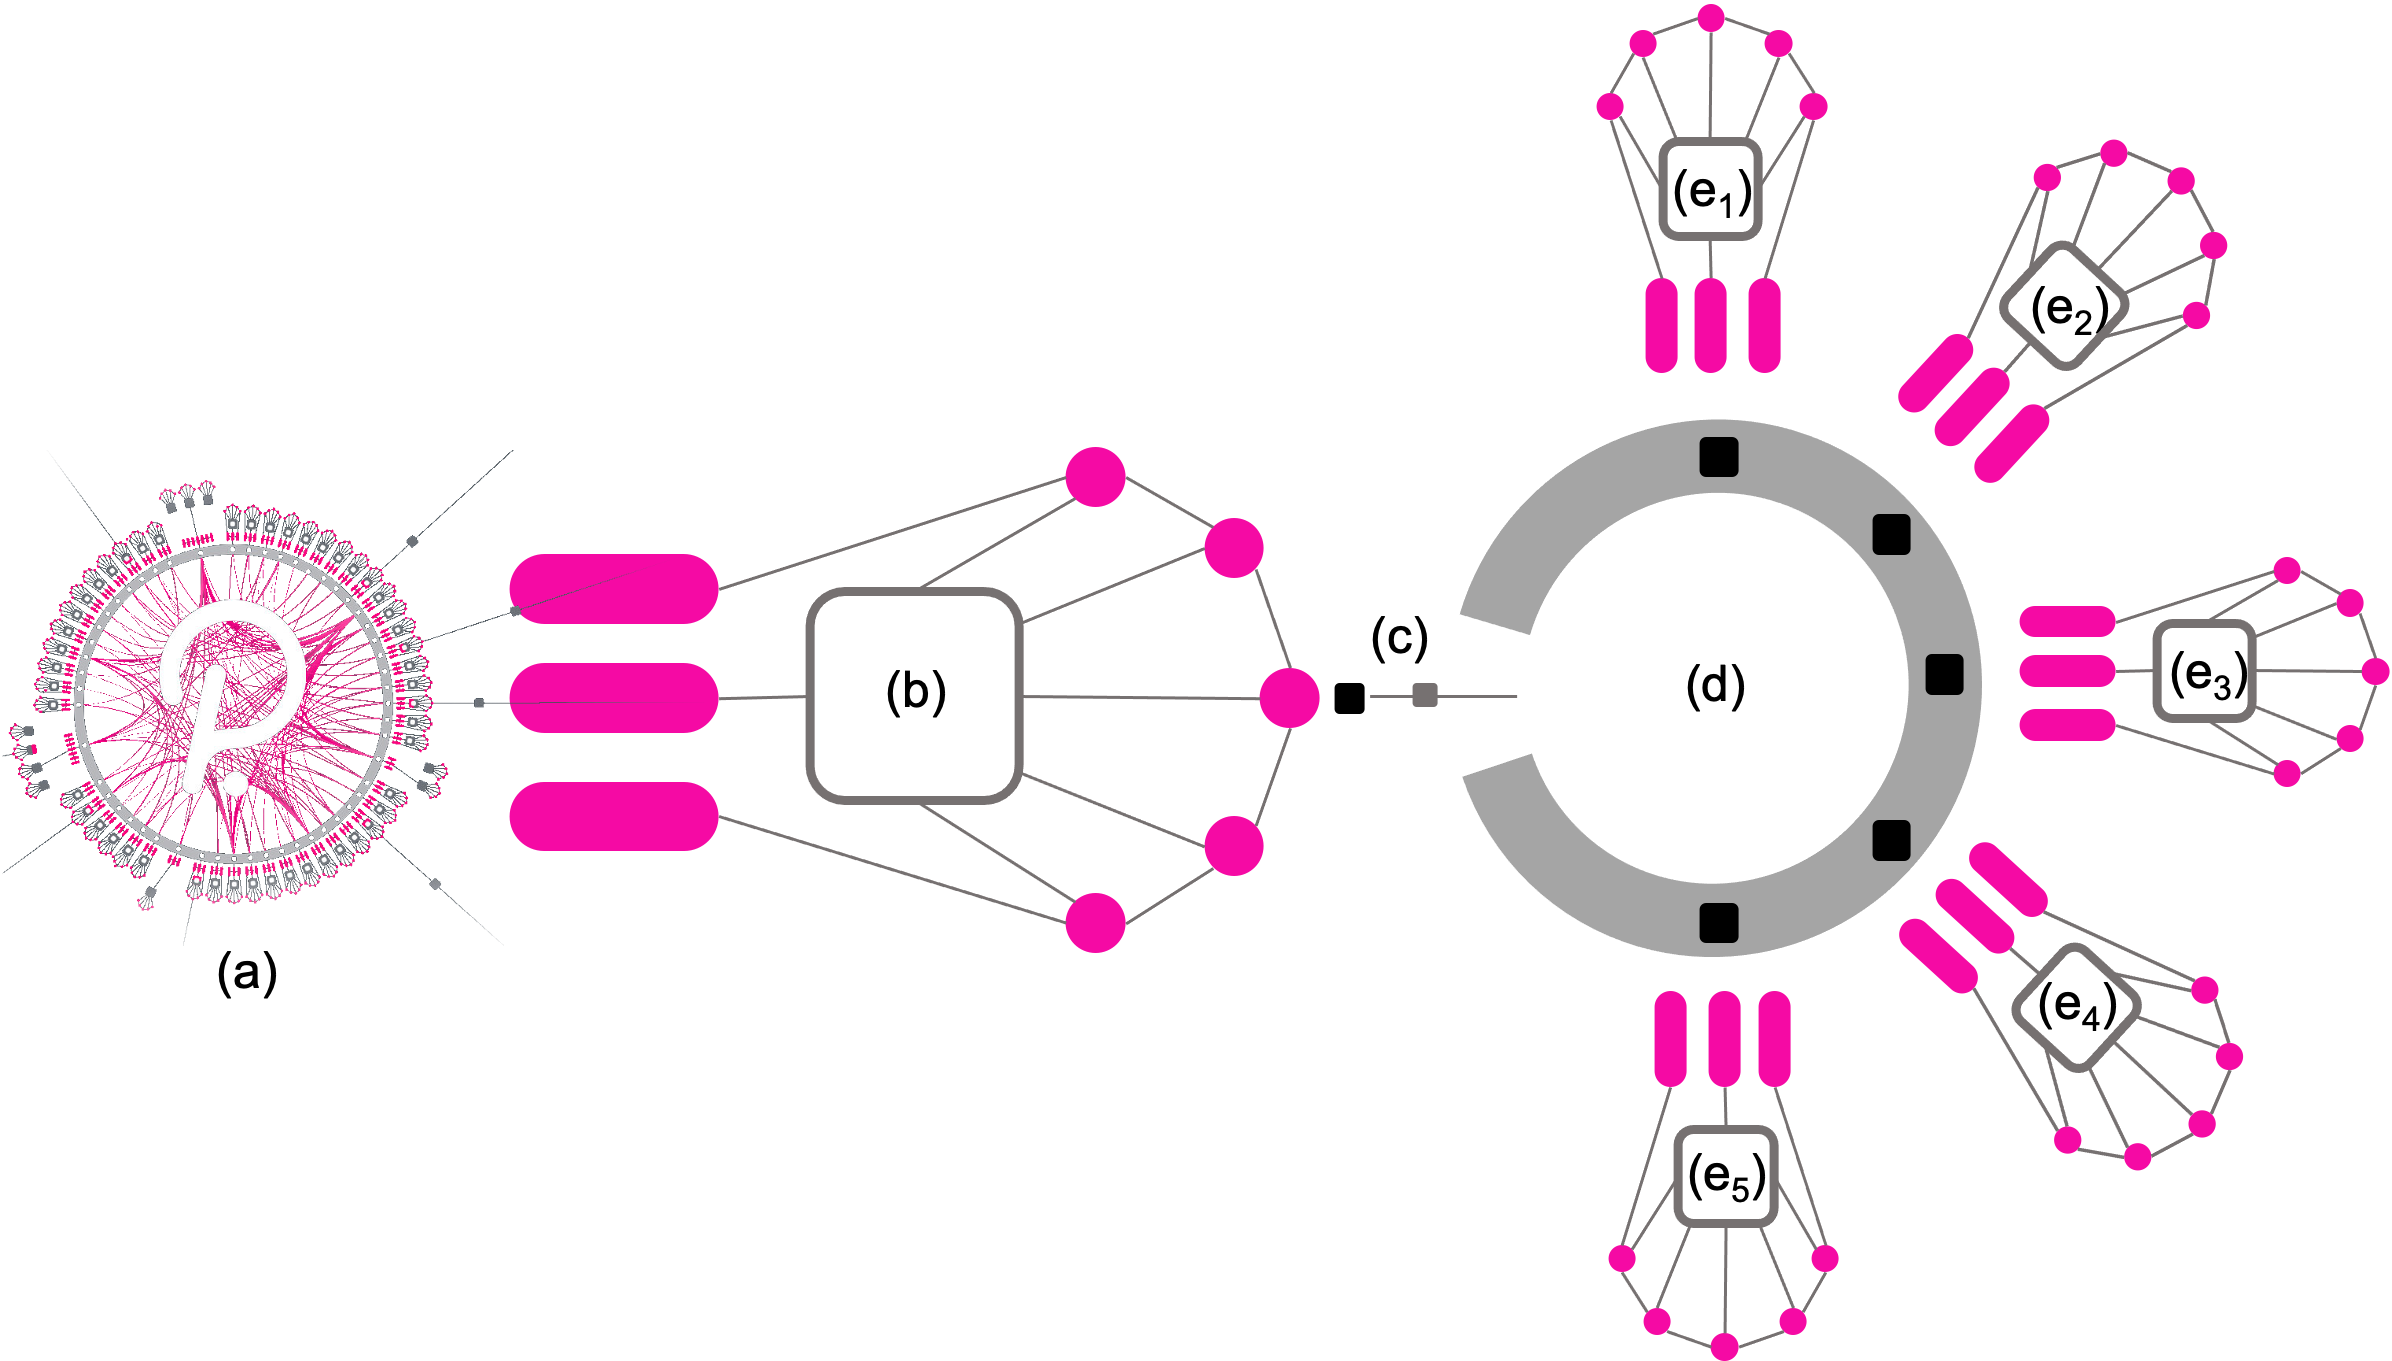
\includegraphics[width=1\textwidth]{phase2.png}
        \captionof{figure}{
            Vision for the design where the set of validators 
            of the previous Evochains gather in the form of a 
            relay chain (d), connected to the Ownership Parachain via
            one single trustless bridge (c), and providing security
            to the Evochains (e$_i$) via the standard Polkadot relay chain 
            consensus. 
        }
    \medskip
    \label{fig:phase2}
\end{Figure}







